\documentclass[11pt]{article}
\usepackage[ngerman]{babel}
\usepackage{float}
\usepackage{graphicx}
\usepackage{hyperref}
\usepackage{cleveref}
\usepackage[%
  backend=biber,
  style=authoryear,
  doi=false,
  sorting=ynt]{biblatex}
\addbibresource{bib.bib}
\author{Maximilian Heim}
\crefname{section}{Kapitel}{Kapitel}
\crefname{figure}{Abbildung}{Abbildung}
\title{Identitäts- und Berechtigungsmanagement}
\begin{document}
\maketitle
\newpage
\tableofcontents
\newpage
\section{Einleitung}
\subsection{Aufgabenstellung}
Diese Seminararbeit wurde im Rahmen der Vorlesung IT-GRC angefertigt. Ziel der Arbeit ist es die in \cref{subsec:forschungsfragen} definierten Forschungsfragen zu beantworten. Die Forschungsfragen zielen darauf ab wichtige Aspekte des betrieblichen Identitäts- und Berechtigungsmanagements im Kontext der IT-GRC zu beleuchten.
\subsection{Forschungsfragen}
\label{subsec:forschungsfragen}
Im Rahmen der Seminararbeit wurden 7 Forschungsfragen definiert, diese sind im Folgenden aufgeführt.
\begin{itemize}
  \item Was versteht man unter den Begriffen \glqq{}Identität\grqq{} sowie \glqq{}Identitätsmanagement\grqq{} und welche Zielstellung wird dabei verfolgt?
  \item Was versteht man unter den Begriffen \glqq{}Berechtigung\grqq{} sowie \glqq{}Berechtigungsmanagement\grqq{} und welche Zielstellung wird dabei verfolgt?
  \item Welche Standards, Methoden, Technologien und Tools lassen sich differenzieren?
  \item Welche Aufgaben und Prozesse sind im Kontext von Identitäts und Berechtigungsmanagement zu bearbeiten?
  \item Welche betrieblichen Anwendungsfälle zeigen die Bedeutung des Identitäts und Berechtigungsmanagements auf?
  \item Wie wird das Identitäts und Berechtigungsmanagement im Kontext der Sicherheit in der Informationstechnik eingesetzt?
  \item Wer hat im Unternehmen typischerweise die Zuständigkeit für Identitäts und Berechtigungsmanagemnt und wer führt diese Aufgaben operativ durch?
\end{itemize}
\section{Grundlagen}
\label{sec:grundlagen}
\subsection{Einordnung}
% fertig
Das Identitäts- und Berechtigungsmanagent ist eine zentrale Disziplin in der Informationssicherheit. Das Identitäts- und Berechtigungsmanagement besteht aus Richtlinien, Prozessen und Technologien zur Verwaltung von Identitäten und Zugriffssteuerung. Identitätsmanagement und Berechtigungsmanagement sind zwei unterschiedliche Disziplinen, jedoch werden diese meist zusammen angewendet. (vgl. \cite{mohammed2017systematic} Seite 1) Es wird häufig zwischen Identitäts- und Berechtigungsmanagement (IAM) und Customer Identitäts- und Berechtigungsmanagement (CIAM) unterschieden. Bei IAM geht es um die Authentifikation und Zugriffskontrolle im Unternehmen. Im Kontrast behandelt das CIAM die Authentifikation und Zugriffskontrolle von Nutzern außerhalb vom Unternehmen. (vgl. \cite{liveretos2022customer} Seite 2)
\subsection{Identität}
% fertig
Um den Begriff Identitätsmanagement zu definieren sollte zuerst der Begriff der Identität definiert werden. In der Philosophie wird Identität über die Ununterscheidbarkeit von Dingen definiert. Nach dem Identitätsprinzip sind zwei Dinge genau dann identisch wenn sich zwischen ihnen keine Unterschiede finden lassen, d.h. zwei Personen oder zwei Computersysteme sind nie identisch. Hierbei geht es um die Fragestellung \glqq{}wer/was bist du?\grqq{}. Im Kontext des Identitätsmanagements handelt es sich hier um digitale Identitäten, d.h. eine Menge an Attributen und Rollen die einer Person, einem IT-System oder einer Anwendung zugeordnet werden können, inklusive einem Bezeichner und Zugangsdaten die zur Nutzung der Identität notwendig sind. Ein Subjekt (Person, System) kann mehreren digitalen Identitäten zugeordnet sein. (vgl. \cite{bertino2010identity} Seite 21-23) Dieser Sachverhalt ist in \cref{fig:identity} dargestellt.
\begin{figure}[H]
  \centering
  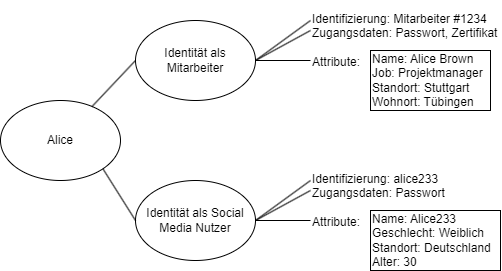
\includegraphics[width=0.9\textwidth]{assets/identity.png}
  \caption{Digitale Identität - Basierend auf Grafik 2.1 aus Identity Management Concepts, Technologies, and Systems von Elisa Bertino und Kenji Takahashi}\label{fig:identity}
\end{figure}
In der Informationstechnik wird der Beweis über die eigene Identität, basierend auf Bezeichner und Zugangsdaten als Authentifizierung bezeichnet. Es haben sich verschiedenste Authentifizierungsverfahren durchgesetzt von denen im Folgenden einige vorgestellt werden. (vgl. \cite{tsolkas2017} Kapitel 7: Zugriffskontrolle über Authentifizierung)
\paragraph{Authentifizierungsverfahren}
\begin{itemize}
  \item Passwörter und Pins sind die wohl bekanntesten Arten der Authentifizierung. Jedoch ist es auch eine der unsichersten Arten da diese gerne mehrfach verwendet werden oder bei unzureichender Länge geknackt werden können
  \item Tokens sind eine andere Art der Authentifizierung die auf Besitz und Wissen basieren und daher sicherer sind wie rein wissensbasierte Verfahren wie Passwörter. Hierbei wird ein Gerät verwendet welches nach Entsperrung mittels Pin/Passwort ein Einmalpasswort ausgibt oder automatisch die Authentifizierung freigibt
  \item Eine weiteres Beispiel für Authentifizierung ist die Biometrie. Hierbei werden z.B. der Fingerabdruck, die Retina oder die Stimme einer Person verwendet um diese zu authentifizieren
\end{itemize}
\subsection{Identitätsmanagement}
Identitätsmanagement ist die Verwaltung von digitalen Identitäten im Zuge der Authentifizierung und Weitergabe von Identitätsinformationen. (vgl. \cite{bertino2010identity} Seite 23) Die Aufgaben im Bereich des Identitätsmanagements sind vielfältig. Es gibt unterschiedliche Definitionen von den Teilbereichen des Identitätsmanagements. Jedoch lassen sich aus den verschiedenen Quellen grundlegende Aufgaben extrahieren welche im Rahmen des Identitätsmanagements durchgeführt werden müssen. Die Aufgabenbereiche sind im Folgenden aufgelistet.
\begin{itemize}
  \item Identity Lifecycle Management: Management von Prozessen für die Provisonierung, Änderung und Deprovisionierung von digitalen Identitäten (vgl. \cite{bertino2010identity} Seite 29-37)
  \item Technologie: Planung, Implementierung und Wartung der Infrastruktur zur Speicherung und Authentifizierung von digitalen Identitäten (vgl. \cite{bertino2010identity} Seite 45)
  \item Compliance: Identifikation von Standards und Gesetzen welche eingehalten werden müssen, Definition von Prozessen zur Einhaltung der Compliance Vorgaben (vgl. \cite{bertino2010identity} Seite 17)
  \item Audit: Auditierung der Compliance Vorgaben im Rahmen der Identifikation von Abweichungen zu den Vorgaben und Speicherung von Transaktionen zur Nachverfolgbarkeit (vgl. \cite{bertino2010identity} Seite 17)
\end{itemize}
\subsection{Berechtigung}
% fertig
Berechtigungen oder auch Zugriffsberechtigungen beschreiben welche Identitäten auf welche Ressourcen zugreifen dürfen. Eine Berechtigung besteht aus einer zu berechtigenden Ressource und aus einer zu berechtigenden Operation für diese Ressource. Beispiele hierfür sind der Schreibzugriff auf eine Datenbank, der Lesezugriff auf Dokumente oder der Konfiguration von Rechnersystemen. (vgl. \cite{tsolkas2017} Seite 3-4) Dieser Prozess findet nach der Authentifizierung statt. Hierbei geht es um die Fragestellung \glqq{}was ist erlaubt?\grqq{}. Die Kontrolle der Berechtigungen basierend auf einer Identität wird Zugriffskontrolle oder auch Autorisierung genannt. (vgl. \cite{tsolkas2017} Seite 161-162)
\subsection{Berechtigungsmanagement}
%fertig
Berechtigungsmanagement ist verantwortlich für die Festlegung welche Nutzer/Entitäten auf welche Ressourcen Zugriff haben und die Kontrolle dieser Berechtigungen. (vgl. \cite{orp4} Seite 1) Das Ziel hierbei ist das Least-Privilege-Prinzip (PoLP) umzusetzen. (vgl. \cite{orp4} Seite 2) Die Definitionen der Aufgabenbereiche im Berechtigungsmanagement divergieren wie auch beim Identitätsmanagement je nach Quelle. Jedoch lassen sich ebenso verschiedene Aufgabenbereiche identifizieren, diese sind im Folgenden vorgestellt.
\begin{itemize}
  \item Berechtigungssteuerung: Management von Prozessen für die Provisonierung, Änderung und Deprovisionierung von Berechtigungen (vgl. \cite{orp4} Seite 1 und \cite{tsolkas2017} Seite 176)
  \item Technologie: Planung, Implementierung und Wartung der Infrastruktur zur Berechtigungskontrolle (vgl. \cite{tsolkas2017} Seite 177)
  \item Compliance: Identifikation von Standards und Gesetzen welche eingehalten werden müssen, Definition von Prozessen zur Einhaltung der Compliance Vorgaben (vgl. \cite{conta2017leitfaden} Seite 10-31)
  \item Audit: Auditierung der Compliance Vorgaben im Rahmen der Identifikation von Abweichungen zu den Vorgaben und Speicherung von Transaktionen zur Nachverfolgbarkeit (vgl. \cite{tsolkas2017} Seite 21)
\end{itemize}
\subsection{Identitäts- und Berechtigungsmanagementsystem}
% fertig
Die systematische Unterteilung von Identitäts- und Berechtigungsmanagement erweist sich als schwierig da es hierbei viele Abhängigkeiten gibt. Ein besseres Gesamtbild ergibt sich durch die Betrachtung der Prozesse im Kontext des kombinierten Identitäts- und Berechtigungsmanagements. In \cref{figure:iam} ist der Ablauf der Zugriffssteuerung im Rahmen eines IAM Systems illustrativ dargestellt.
\begin{figure}[H]
  \centering
  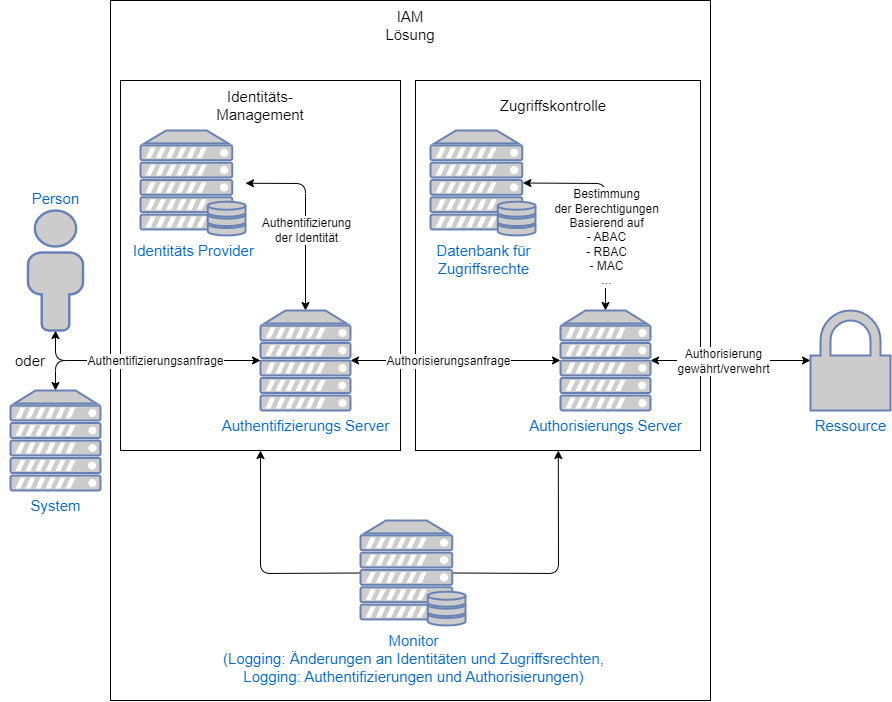
\includegraphics[width=0.9\textwidth]{assets/accessmanagement2.png}
  \caption{Illustration der Zugriffssteuerung im Rahmen eines IAM Systems - Basierend auf Grafik 1 aus Identity and access management using distributed ledger technology: A survey von Fariba Ghaffari, Komal Gilani, Emmanuel Bertin und Noel Crespi}\label{figure:iam}
\end{figure}
\subsection{Erkenntnisse im Kontext von IT-GRC}
% fertig
\begin{itemize}
  \item Die Nutzung von Identitäts- und Berechtigungsmanagement spielt eine zentrale Rolle im unternehmensweiten Sicherheitsmanagement. Durch die Steuerung welche logischen Identitäten auf welche Ressourcen zugreifen kann können eine Vielzahl an beabsichtigter und unbeabsichtigter Sicherheitsrisiken minimiert werden.
  \item Das Identitäts- und Berechtigungsmanagement ist ein tiefgreifendes Thema in der IT-Governance und besteht aus verschiedenen Prozessen, Technologien und Gesetzen welche im Kontext der gesamten Unternehmenstätigkeiten betrachtet werden müssen.
\end{itemize}
\section{Methoden, Technologien und Tools}
\label{sec:existing}
\subsection{Betriebliche Motivation}
% motiviation für den einsatz von methoden, tools und technologien
Der Einsatz von eigens entwickelten Methoden, Technologien und Tools birgt eine Vielzahl an Problemen. So z.B. hohe Kosten oder Sicherheitsprobleme. Hierbei ist es von Vorteil auf etablierte Methoden, Technologien und Tools zu setzen. Standardisierte Methoden wie der IT-Grundschutz oder die NIST 800-53A definieren Vorgehensweisen um die Gefahrenlage gezielt zu bewältigen, standardisierte Technologien wie SAML oder OAuth unterstützen die interoperable Implementierung von Identitäts- und Berechtigungsmanagement und ausgereifte Produkte bieten eine ganze Bandbreite an Funktionalitäten. Im Folgenden werden daher einige Methoden, Tools und Technologien vorgestellt.
\subsection{Standardisierte Methoden}
\paragraph{BSI}
%fertig
Das Bundesamt für Sicherheit der Informationstechnik (BSI) definiert den IT-Grundschutz. Dieser besteht aus den BSI-Standards und dem IT-Grundschutz-Kompendium. (vgl. \cite{bsi2017grundschutz}) In BSI-Standard 200-1 werden Sicherheitsmaßnahmen definiert die zur Behandlung der Risiken geeignet sind, in diesen Sicherheitsmaßnahmen wird das Identitäts- und Berechtigungsmanagement als Sicherheitsmaßnahme aufgeführt. (vgl. \cite{bsi20172001} Seite 35) In Bezug auf den BSI-Standard definiert das IT-Grundschutz-Kompendium Prozessbausteine zur Umsetzung des ISMS.(vgl. \cite{bsi2023kompendium}) Hier wird im Prozessbaustein \glqq{}ORP.4 Identitäts- und Berechtigungsmanagent\grqq{} auf verschiedene Anforderungen für die Umsetzung von Identitäts- und Berechtigungsmanagement eingegangen. Kapitel 3.1 definiert Basis-Anforderungen welche umgesetzt werden müssen. Kapitel 3.2 definiert Standard-Anforderungen welche umgesetzt werden sollten. Kapitel 3.3 definiert Anforderungen welche bei erhöhtem Schutzbedarf umgesetzt werden sollten. (vgl. \cite{orp4}) Zusätzlich zu ORP.4 gibt es das Dokument \glqq{}Umsetzungshinweise zum Baustein: ORP.4. Identitäts- und Berechtigungsmanagement\grqq{} welches spezifische Maßnahmen zur Umsetzung von ORP.4 definiert. (vgl. \cite{bsi2022umsetzungshinweiseorp4})
\paragraph{ISO 27001 Annex A.9}
%fertig
ISO 27001 definiert mit Anhang A.9 Kontrollen für die Zugangskontrolle. Das Kapitel ist in die Unterkapitel \glqq{}9.1 Geschäftsanforderungen an die Zugangssteuerung\grqq{}, \glqq{}9.2 Benutzerzugangsverwaltung\grqq{}, \glqq{}9.3 Benutzerverantwortlichkeiten\grqq{} und \glqq{}9.4 Zugangssteuerung für Systeme und Anwendungen\grqq{} unterteilt. (vgl. \cite{kersten2020iso27001} Seite 121-138) Die Maßnahmen des oben erwähnten IT-Grundschutz-Kompendiums eignen sich zur Umsetzung der ISO 27001 Kontrollen. Somit kann eine ISO 27001 Zertifizierung auf Basis vom IT-Grundschutz umgesetzt werden. (vgl. \cite{bsi2023iso27001basis}) Eine Gegenüberstellung des Anhangs A.9 zu den Prozessbausteinen lässt sich im Dokument \glqq{}Zuordnungstabelle: Zuordnung ISO/IEC 27001 zum IT-Grundschutz\grqq{} finden. (vgl. \cite{bsi2021map})
\paragraph{ISO/IEC 24760}
%fertig
Eine speziell für Identitätsmanagement erstellte Norm ist die ISO/IEC 24760. Hierbei werden Konzepte und operative Strukturen zur Umsetzung von Identitätsmanagement definiert. Die Norm geht hierbei auf die Provisionierung, Administration und Nutzung von digitalen Identitäten ein, die digitalen Identitäten sind im Kontext der Norm nicht nur Personen sondern auch Organisationen oder IT-Systeme. (vgl. \cite{iso2019idm} \glqq{}Introduction \grqq{})
\paragraph{NIST 800-53A}
%fertig
Das National Institute of Standards and Technology (NIST) publizierte die \glqq{}NIST Special Publication 800-53A - Assessing Security and Privacy Controls in Information Systems and Organizations\grqq{}. Dieses Dokument stellt Prozesse und Methoden für die Bewertung von Sicherheits- und Datenschutzmaßnahmen vor. Im Kapitel \glqq{}Security and Privacy Assessment Procedures\grqq{} wird im Unterkapitel 4.1 \glqq{}Access Control Family (AC)\grqq{} auf Zugangskontrolle und im Unterkapitel 4.7 \glqq{}Identification and Authentication Family (IA)\grqq{} auf Identifizierung und Authentifizierung eingegangen. (vgl. \cite{nist202280053a})
\subsection{Methoden}
\paragraph{Föderiertes Identitätsmanagement}
Föderiertes Identitätsmanagement (FIdM) ist eine Lösung für fragmentierte Identitätsinformationen. So hatte in der Vergangenheit jeder Service einen eigenen Identitätsprovider. Dies führt zu schlecht zu wartenden Identitätsinformationen und Sicherheitsproblemen denn die Anzahl der Sicherheitsrisiken wächst mit der redundanten Speicherung der Informationen. Aus diesem Grund wurde das Konzept der Föderierten Identität eingeführt. Hierbei werden sogenannte \glqq{}trust relationships\grqq{} unter Identity Providern (IdP) und Service Providern (SP) beschlossen um eine zentrale Verwaltung von Identitäten umzusetzen. Dieser Sachverhalt ist in \cref{fig:fidm} dargestellt. (vgl. \cite{cantor2003liberty} Seite 4-6)
\begin{figure}[H]
  \centering
  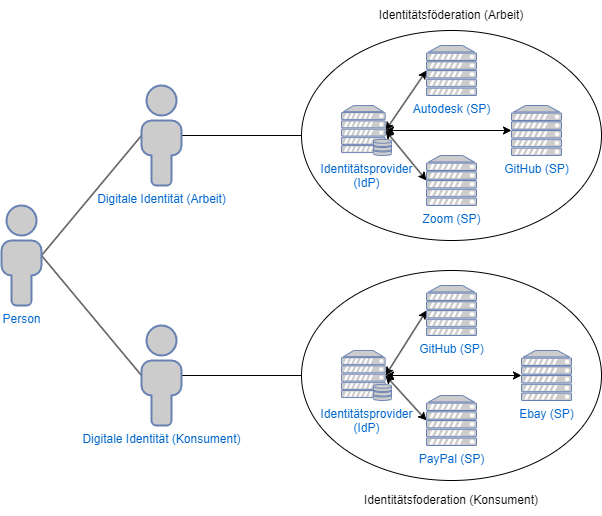
\includegraphics[width=0.9\textwidth]{assets/federated.png}
  \caption{Föderiertes Identitätsmanagement - Basierend auf Grafik 2 aus Liberty ID-FF Architecture Overview von Scott Cantor, Jeff Hodges, John Kemp und Peter Thompson}\label{fig:fidm}
\end{figure}
\paragraph{Single Sign On}
Single Sign On (SSO) ist ein auf FIdM basierendes Konzept. Hierbei werden nach einmaliger Authentifizierung bei einem Service Provider im Rahmen einer Identitätsföderation automatisiert die Authentifizierungsinformationen lokal gespeichert. Wenn der Nutzer anschließend einen anderen Service Provider nutzen möchte wird dieser automatisch authentifiziert, dies führt zu einer besseren Nutzerfreundlichkeit. (vgl. \cite{cantor2003liberty} Seite 23-24)
\paragraph{Multi Faktor Authentifizierung}
Es gibt 3 verschiedene Arten von Informationen die für die Authentifizierung verwendet werden können. Wissen, Besitz und Biometrie. Die Unterscheidung der Faktoren ist in \cref{figure:mfa} dargestellt.
\begin{figure}[H]
  \centering
  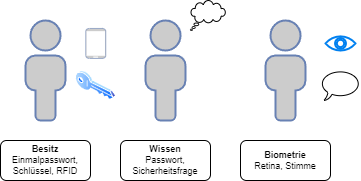
\includegraphics[width=0.7\textwidth]{assets/mfa.png}
  \caption{Faktoren zum Identitätsnachweis - Basierend auf Grafik 1 aus Multi-Factor Authentication: A Survey von Aleksandr Ometov 1, Sergey Bezzateev, Niko Mäkitalo, Sergey Andreev, Tommi Mikkonen und Yevgeni Koucheryavy}\label{figure:mfa}
\end{figure}
In der Vergangenheit wurde meistens nur eine Ein-Faktor Authentifizierung durchgeführt, d.h. eine Person musste eine Chipkarte oder ein Passwort zur Authentifizierung vorweisen. Mit steigenden Bedenken der Sicherheit ging dieser Ansatz in Richtung der Mehr-Faktor Authentifizierung über. So verwenden viele Anwendungen heutzutage 2 oder sogar 3 Faktoren. Dies erhöht die Sicherheit der Anwendungen signifikant. (vgl. \cite{ometov2018multi} Seite 1-4)
\subsection{Prozesse}
\paragraph{Identitäts Lebenszyklus}
%fertig
Ein zentraler Prozess welcher im Rahmen des Identitätsmanagements definiert und umgesetzt werden muss ist der Identitäts Lebenszyklus. Dieser enthält die grundlegenden Elemente Geburt, Leben, Änderung, Tod und Governance. Der Prozess ist in \cref{fig:idlc} dargestellt und wird nachfolgend genauer beschrieben. (vgl. \cite{bertino2010identity} Seite 29-37 (ganzer Paragraph))
\begin{figure}[H]
  \centering
  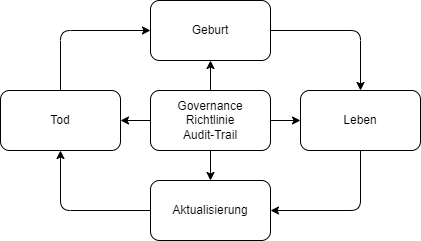
\includegraphics[width=0.6\textwidth]{assets/idlc.png}
  \caption{Identity Life Cycle - Basierend auf Grafik 2.3 aus Identity Management Concepts, Technologies, and Systems von Elisa Bertino und Kenji Takahashi}\label{fig:idlc}
\end{figure}
\subparagraph{Geburt}
\begin{itemize}
  \item Datensammlung \& Verifikation: Der erste Schritt in der Geburt einer Identität ist die Sammlung relevanter Attribute wie Name, Geburtsdatum, Wohnsitz, Rolle im Unternehmen etc. und Überprüfung dieser.
  \item Zugangsdaten: Um dem Subjekt Zugriff auf die provisionierte Identität zu geben müssen Bezeichner (z.B. E-Mail Addressen oder Nutzernamen) und geeignete Verfahren zur Authentifikation festgelegt werden. So werden in diesem Schritt z.B. Einmalpasswörter für die initiale Anmeldung vergeben oder der Fingerabdruck der zu authentifizierenden Person gespeichert.
  \item Erstellung: Nachdem alle relevanten Informationen zur Erstellung der Identität gesammelt wurden kann die Identität erstellt werden.
\end{itemize}
\paragraph{Leben}
\begin{itemize}
  \item Authentifizierung: Die Authentifizierung der eignenen Identität ermöglicht die gesicherte Nutzung von Ressourcen. Sie sind eine zentrale Komponente im Leben einer Identität.
  \item Teilen von Attributen: Verfahren zur Weitergabe von Informationen sind ein zentraler Aspekt beim Ausleben einer digitalen Identität.
\end{itemize}
\paragraph{Aktualisierung}
\begin{itemize}
  \item Attributsänderung: Bei Änderung von Attributen wie z.B. Rollen im Unternehmen, Wohnort oder Namensänderung müssen die Attribute schnellstmöglich aktualisiert werden um die Integrität dieser zu gewährleisten.
  \item Urlaub/Krankheit: Eine wenig diskutierte aber sinnvoll erscheinende Änderung an Identitäten ist der Entzug von Berechtigungen während dem Urlaub oder Krankheit. Somit können nicht genutzte Berechtigungen für IT Systeme und Zugänge entzogen werden, andernfalls kann dies ein grundloses Risiko darstellen. (vgl. \cite{tsolkas2017} Seite 44)
  \item Zugangsdatenänderung: Zugangsdaten wie neu ausgestellte Zertifikate oder geänderte Passwörter müssen ebenso aktualisiert werden um die Authentifizierung zu gewährleisten.
\end{itemize}
\paragraph{Tod}
\begin{itemize}
  \item Kündigung: Bei der Kündigung von Mitarbeitern oder bei der Dekommisionierung von Systemen muss der Zugriff auf Ressourcen aufgehoben werden um Sicherheitsrisiken zu verhindern. In diesem Szenario ist es jedoch auch wichtig die Identitätsinformationen weiterhin zu persistieren um für zukünftige Untersuchungen wie z.B. des Audit-Trails eine Zuordnung zu haben.
\end{itemize}
\paragraph{Governance}
\begin{itemize}
  \item Governance Richtlinien: Die Administration, Nutzung und Weitergabe von Identitätsinformationen muss klar durch Richtlinien definiert sein.
  \item Audit-Trail: Jegliche Transaktionen bezüglich Zugriff, Änderung oder Weitergabe von Identitätsinformationen sollten aufgezeichnet werden um die Rückverfolgbarkeit zu gewährleisten.
\end{itemize}
\paragraph{Audit}
Ein weiterer zentraler Prozess im Identitäts- und Berechtigungsmanagement ist die Auditierung des Ist-Zustands. Hierbei müssen verschiedenste Prozesse im Unternehemen dokumentiert und anschließend auf Konformität geprüft werden um Abweichungen vom Soll-Zustand zu identifizieren. Dabei muss auf verschiedenste Aspekte eingegangen werden, von diesen sind im Folgenden einige aufgeführt. (vgl. \cite{devlekar2022identity} Seite 397-398, \cite{tsolkas2017} Seite 123-124, 193, 204. \cite{haag2012selecting} Seite 8)
\begin{itemize}
  \item Sicherstellung der Funktionstrennung
  \item Analyse der Audit-Logs (Änderungen an Identitäten und Berechtigungen)
  \item Compliance mit Standards und Gesetzen
  \item Sicherheit der involvierten Technik
\end{itemize}
\subsection{Technologien}
Es existieren einige standardisierte Technologien die im Kontext vom Identitäts- und Berechtigungsmanagement eingesetzt werden.
\paragraph{SAML}
SAML ist ein weit verbreiteter Standard zur Umsetzung von Sicherheits-Assertationen im Kontext von Identitätsföderationen. Mit SAML wird ein XML Format definiert welches zur Authentifizierung und Authorisierung von Nutzern verwendet werden kann. Im Kontext von SAML werden verschiedene Begriffe definiert. (vgl. \cite{hughes2005security} Seite 5-10)
\begin{itemize}
  \item Assertation - Eine Assertation über die Charakteristiken und Attribute eines Subjekts. So z.B. die Zugehörigkeit zu einer Gruppe oder der Besitz eines Attributs.
  \item Identity Provider (IdP) - Der Server der für die eigentliche Bearbeitung der Assertation zuständig ist. Er erhält die Anfrage und leitet die Antwort an den Service Provider weiter.
  \item Service Provider (SP) - Das Ziel der Authentifizierung/Authorisierung, dieser stellt eine Ressource/Service zur Verfügung.
\end{itemize}
\paragraph{OAuth}
OAuth ist eine verbreiteter Standard zur delegierten Zugriffskontrolle welcher in RFC 6749 definiert wird. Das Ziel hierbei ist das Problem der Autorisierung Dritter zu lösen. Somit müssen keine sensiblen Informationen wie Passwörter mit Dritten geteilt werden um ihnen Zugriff auf eine Ressource zu geben. Im Kontext des Standards werden folgende Begriffe definiert.
\begin{itemize}
  \item Ressourcenbesitzer - Eine Entität welche die Ressource besitzt und Zugriff gewähren kann
  \item Ressourcenserver - Ein Server welcher die Ressource hostet und auf Anfragen mittel Zugriffstokens reagieren kann
  \item Klient - Eine Anwendung welcher für Ressourcen authorisiert ist und Anfragen an den Ressourcenserver senden kann
  \item Authorisierungsserver - Ein Server welcher Zugriffstokens im Name des Ressourcenbesitzers an den Klient ausstellen kann
\end{itemize}
Der Ablauf des Protokolls ist in Grafik~\cref{fig:oauth} abgebildet. (vgl. \cite{rfc6749})
\begin{figure}[H]
  \centering
  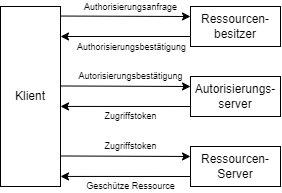
\includegraphics[width=0.6\textwidth]{assets/oauth.png}
  \caption{Protokoll OAuth 2.0 - Basierend auf RFC 6749}\label{fig:oauth}
\end{figure}
\paragraph{OpenID}
OpenID Connect (OIDC) ist ein auf OAuth 2.0 basierender Standard für föderierte Authentifizierung welches die veraltete OpenID 2.0 Spezifikation ablößt. Somit kann im Rahmen des Identitätsmanagements ein zentraler OpenID Provider (OP) über ein REST API zur Authentifizierung und SSO eingesetzt werden. (vgl. \cite{naik2017choice} Seite 6-9)
\paragraph{Einordnung SAML, OAuth, OIDC}
\begin{itemize}
  \item SAML und OIDC werden beide als Technologie für Authentifizierung und Authorisierung im Kontext von FIdM eingesetzt, beide Ermöglichen die Umsetzung von SSO. SAML wird hierbei eher im Unternehmenkontext und OIDC im Konsumentenkontext verwendet
  \item OAuth wird für die Authorisierung Dritter im Kontext von FIdM genutzt
\end{itemize}
(vgl. \cite{naik2017choice})
\subsection{Tools}
IAM Lösungen ersetzen nicht die Einhaltung von Standards und die sorgfältige Planung von IAM Prozessen. Sie sind jedoch hilfreiche Werkzeuge zur technischen Umsetzung von IAM. Zur konkreten Umsetzung in Organisationen gibt einige quelloffene Lösungen und von den großen Technologiekonzernen wie Microsoft, SAP, IBM, Oracle werden kommerzielle Lösungen angeboten. Im Folgenden werden quelloffene und kommerzielle Produkte vorgestellt welche bei der Umsetzung von CIAM und IAM verwendet werden können.
\paragraph{Shibboleth}
%fertig
Shibboleth ist eine auf SAML basierende, quelloffene Lösung zur Umsetzung von föderierter Identität. Shibboleth kann in diesem Kontext als Identity Provider und Service Provider verwendet werden. Somit kann eine SSO Integration von verschiedensten Anwendungen realisiert werden. (vgl. \cite{kamal2015shibboleth} Kapitel 5) Die Technologie setzt sich aus 4 Software Paketen zusammen. Die Softwarepakete sind hierbei der Identity Provider, Service Provider, Embedded Discovery Service und der Metadata Aggregator. Der Embedded Discovery Service erlaubt einem SP mehrere IdP's zur Verfügung zu stellen. Der Metadata Aggregator erlaubt die dynamische Abfrage von Metadaten vom Identity Provider (vgl. \cite{shibboleth2024software})
\paragraph{IBM Security Verify}
%fertig
IBM bietet mit dem Produkt \glqq{}IBM Security Verify\grqq{} eine Cloud basierte Lösung zum Identitäts- und Berechtigungsmanagement und Customer Identitäts- und Access Management an. Dieses Produkt bietet umfangreiche Funktionalitäten wie SSO, MFA, Consent Management. Zudem wird die Funktion Identity Analytics angeboten, d.h. die automatische Analyse von Identitäten und Berechtigungen zum Zweck der Identifizierung von Abweichungen. (vgl. \cite{ibm2024verify})
\paragraph{Microsoft Entra ID}
Microsoft bietet mit dem Produkt \glqq{}Microsoft Entra ID\grqq{} eine Cloud basierte Lösung zum Identitäts- und Berechtigungsmanagement von Microsoft und drittpartei Diensten an. Dieses Produkt bietet Funktionen wie z.B. Multi-Faktor-Authentifizierung mittels Microsoft Authenticator.
\paragraph{SAP Cloud Identity Access Governance}
SAP bietet mit dem Produkt \glqq{}SAP Cloud Identity Access Governenace\grqq{} eine Cloud basierte Lösung zum Identitäts- und Berechtigungsmanagement an.
\paragraph{Okta Inc.}
Das Unternehmen Okta Inc. ist ein in den USA ansässiges Unternehmen welches sich auf IAM spezialisiert hat. Mit rund 6000 Mitarbeitern und mehr als einer Milliarde US-Dollar an Umsatz ist es ein führender Hersteller von IAM Produkten. Vom Unternehmen werden 2 Produkte angeboten. Customer Identity Cloud und Workforce Identity Cloud. Customer Identity Cloud ist eine Lösung zum Customer Identity Management, d.h. es ermöglicht die sichere Verwaltung und Authentifizierung von Kunden-Identitäten. Workforce Identity Cloud ist eine Lösung zum Unternehmensinternen Identitäts- und Berechtigungsmanagement.
\subsection{Erkenntnisse im Kontext von IT-GRC}
\begin{itemize}
  \item Es existieren eine Vielzahl an normativen Standards wie ISO 27001, IT-Grundschutz und NIST 800-53A welche nach Identitäts- und Berechtigungsmanagement fordern und Umsetzungshinweise definieren
  \item Professionelle IAM Lösungen können durch eine Vielzahl an Funktionalitäten dazu beitragen Identitäts- und Berechtigungsmanagement effizient umzusetzen.
  \item Es existiert eine Vielzahl an Technologien welche eine interoperable Umsetzung von Identitäts- und Berechtigungsmanagement ermöglichen
\end{itemize}
\section{Betriebliches Identitäts- und Berechtigungsmanagement}
\label{sec:betrieb}
\subsection{Überblick}
\subsection{Organisatorische Aspekte}
Im Rahmen der Ausarbeitung eines IAM Konzepts im Unternehmen müssen hierbei klare Verantwortlichkeiten, Prozesse und Technologien definiert werden. Die relevanten Organisationseinheiten zum Identitäts- und Berechtigungsmanagement werden im Folgenden vorgestellt.
\paragraph{Führungebene}
%fertig
IAM fällt unter die Domäne der Informationssicherheit, benötigt jedoch gegebenfalls umfangreiche IT Infrastruktur und Produkte. Auf der Führungsebene im Unternehmen sind daher der Chief Information Security Officer (CISO) und der Chief Information Officer (CIO) für die Umsetzung des Identitäts- und Berechtigungsmanagement verantwortlich. (vgl. \cite{mont2010economics} Seite 1)
\paragraph{IT-Betrieb}
Im Unternehmen sind CIO und CISO zwar für das Identitäts- und Berechtigungsmanagement grundlegend verantwortlich, nicht jedoch für die operative Umsetzung dieses. Daher sind dem CIO und CISO möglicherweise ein oder mehrere Administratoren unterstellt welche die Implementierung und Wartung der Systeme im Kontext des Identitäts- und Berechtigungsmanagements bewerkstelligen. (vgl. \cite{microsoft2024iamadmin})
\paragraph{Helpdesk}
%fertig
Der Helpdesk ist im Unternehmen eine zentrale Anlaufstelle für Probleme mit der Authentifizierung wie vergessener Passwörter oder fehlender Berechtigungen. So wurde bei Umfragen festgestellt dass je nach Unternehmen 10-66 \% aller Helpdesk Tickets aufgrund von vergessener Passwörter erstellt werden. (vgl. \cite{ylen2004centralized} Seite 31, \cite{tsolkas2017} Seite 189-190, \cite{hummer2016adaptive} Seite 11) Ein wichtiger Aspekt hierbei ist die Einhaltung fester Prozesse welche mögliche Angriffe durch Social Engineering verhindern. (vgl. \cite{wood2005implementing}, \cite{ylen2004centralized} Seite 26)
\paragraph{Personalabteilung}
%fertig
Eine Zentrale Rolle im Identity Life Cycle spielt die Personalabteilung. Dieses ist für die erstmalige Erstellung der Identitäten, der Ausgabe von Authentifizierungsinformationen, der Vergabe von Rollen für rollenbasierte Zugriffskontrolle und der Deprovisionierung bei Beurlaubung und Kündigung zuständig. (vgl. \cite{mohammed2017systematic} Seite 3) So bietet z.B. Microsoft Entra ID oder Okta Workforce Identity eine direkte Integration von HR Anwendungen in den Identitäts Lebenszyklus an. (vgl. \cite{oktahr}, \cite{Billmath2024})
\subsection{Technische Aspekte}
%fertig
Für die Umsetzung von Identitäts- und Berechtigungsmanagement im Betrieb bieten sich die Lösungen der namhaften Hersteller wie Microsoft, SAP oder Okta an. Dies sind ausgereifte Lösungen mit einer Vielzahl an Funktionalitäten die die Umsetzung des Identitäts- und Berechtigungsmanagements unterstützen. Während der traditionelle Ansatz die Nutzung von On-Premise Services war bewegt sich die IAM Industrie in Richtung von SaaS Modellen. Im Kontext von IAM werden diese Lösungen als IDaaS bezeichnet. (vgl. \cite{kunz2014analyzing} Seite 274, \cite{tsolkas2017} Seite 223-224)
\subsection{Wirtschaftliche und rechtliche Aspekte}
Die Signifikanz von Identitäts- und Berechtigungsmanagement in Unternehmen ist tiefgreifend. Es lassen sich mehrere Aspekte identifizieren. Unter anderem Security, Produktivität, Compliance, Wettbewerbsvorteil durch Zertifizierungen und Kundenerlebnis. Diese Aspekte sind im Folgenden aufgeführt.
\paragraph{Security}
%fertig
Die wirtschaftlichen Schäden durch Datendiebstahl und unautorisierte Kontrolle sind immens und steigen stetig. (vgl. \cite{furnell2020understanding} Seite 154) Wenn ein Mitarbeiter eine Vielzahl an Passwörtern für die unternehmensinternen/unternehmensexternen Dienste verwalten muss kann dies zur unsachgemäßen Handhabung führen - so z.B. Notizen mit Passwörtern oder die Verwendung von schwachen Passwörtern, dies erhöht die Wahrscheinlichkeit von Sicherheitrisiken. (vgl. \cite{haag2012selecting} Seite 6-8) Im Jahr 2017 fiel Deloitte einem Cyberangriff zum Opfer. Hierbei wurden sensible Daten geklaut. Grund für den Cyberangriff war ein Administratoraccount ohne Zugriffsbeschränkungen welcher nur mittels Passwort, ohne MFA geschützt war. (vgl. \cite{deloitte2017}) Mittels fest definierter Prozesse des Identitäts Lebenszyklus und der Zugriffssteuerung und Auditierung dieser können Risiken für ähnliche Angriffe minimiert werden.
\paragraph{Produktivität}
%fertig
Im vorherigen Abschnitt wurde die sicherheitstechnische Signifikanz von Identitäts- und Berechtigungsmanagement aufgezeigt. Dies kann jedoch einen negativen Einfluss auf die Produktivität von Mitarbeitern haben. So führt z.B. die Verwendung von mehreren verschiedenen Systemen, alle mit unterschiedlichen Authentifizierungsverfahren dazu dass Mitarbeiter verschiedene Passwörter verwalten müssen oder sich in jedem System separat authentifizieren müssen. (vgl. \cite{radha2012survey} Seite 138, \cite{haag2012selecting} Seite 8-9) Ein weiterer Aspekt sind vergessene Passwörter mit Unterbrechungen im Arbeitsablauf und hohem Helpdesk aufwand. Mit der Anwendung von SSO Verfahren lässt sich dieser Aufwand auf ein Minimum reduzieren. (vgl. \cite{thakur2015user} Seite 2-3, \cite{haag2012selecting} Seite 8-9) ährend die Umsetzung des Principle of Least Privilege wünscheswert ist können schlecht konfigurierte Zugriffsberechtigungen dazu führen dass Mitarbeiter ihre Arbeit unterbrechen müssen um neue Rechte anzufordern. Dies kann unter Umständen zu teuren Verzögerungen im direkten Arbeitsablauf adminstrativer oder operativer Aufgaben führen. (vgl. \cite{weishaupl2015towards} Seite 1-1)
\paragraph{Kundenerlebnis}
%fertig
Im Kontext des Customer IAM führen ungeeignete IAM Lösungen zu erhöhter Komplexität für den Nutzer. Eine strikte Umsetzung von starken Passwörtern oder die Nutzung einer weiteren MFA-App kann für den Kunden abschreckend sein. (vgl. \cite{azhar2014economics} Seite 545, \cite{liveretos2022customer} Seite 472) Somit steigt der Kunde möglicherweise zur Konkurrenz um. Durch das Anbieten von SSO mittels beliebter externer Dienste (Google, Github, Facebook) lässt sich die Komplexität und das Risiko von Sicherheitsproblemen reduzieren.
\paragraph{Wettbewerbsvorteil durch Zertifizierungen}
%fertig
Zertifizierungen mit Sicherheitsstandards wie der ISO 27001 können zu einem Wettbewerbsvorteil führen denn diese sind für Kunden ein möglicher Indikator für Qualität. (vgl. \cite{dobrin2015quality} Seite 1071-1072) Somit kann die Umsetzung von Identitäts- und Berechtigungsmanagement im Rahmen einer ISO 27001 Zertifizierung zu einem Wettbewerbsvorteil führen.
\paragraph{Compliance}
\subparagraph{EuroSOX}
%fertig
Die Richtlinie 2006/43/EG, durch den direkten Bezug zum Sarbanes Oxley Act auch EuroSOX genannt fordert im Rahmen des Internen Kontrollsystems (IKS) nach einer Berechtigungsvergabe und Funktionstrennung im Unternehmen. Dies stellt eine direkte Forderung für Identitäts- und Berechtigungsmanagement dar. (vgl. \cite{conta2017leitfaden} Seite 15)
\subparagraph{KonTraG}
%fertig
Das KonTraG fordert Unternehmen auf ein Risikomanagementsystem zu implementieren. Unauthorisierter Zugriff auf sensible Daten und Geschäftsprozesse kann in diesem Kontext als Risiko aufgefasst werden. D.h. es besteht eine indirekte Forderung nach Identitäts- und Berechtigungsmanagement. (vgl. \cite{conta2017leitfaden} Seite 16-17)
\subparagraph{BDSG}
Im BDSG nimmt Identitäts- und Berechtigungsmanagement eine zentrale Rolle ein. (vgl. \cite{conta2017leitfaden} Seite 21-24)
\begin{itemize}
  \item Zutrittskontrolle, Zugriffskontrolle: Systeme die personenbezogene Daten verarbeiten müssen vor unauthorisiertem Zutritt und Zugriff geschützt werden. Dies stellt eine direkte Forderung für physische und logische Berechtigungskontrollen dar.
  \item Weitergabekontrolle: Beim Transport von personenbezogenen Daten muss die Vertraulichkeit und Integrität der Daten gewährleistet sein.Jegliche Transaktionen müssen protokolliert werden. Dies stellt eine direkte Forderung für Audit-Trails und Berechtigungskontrollen dar.
  \item Eingabekontrolle: Bei der Erfassung von personenbezogenen Daten muss die Nachvollziehbarkeit des Ursprungs gewährleistet sein. Dies stellt eine direkte Forderung für Audit-Trails dar.
\end{itemize}
\paragraph{EU-DSGVO}
%fertig
Die DSGVO stellt verschiedenste Forderungen für die sichere Erhebung, Speicherung und Verarbeitung von personenbezogener Daten. (vgl. \cite{Hindle_2020}, \cite{eu2016})
\begin{itemize}
  \item Artikel 5 - Grundsätze für die Verarbeitung personenbezogener Daten - Paragraph 1.f: Die Integrität und Vertraulichkeit personenbezogene Daten muss gewährleistet sein. Somit müssen geeignete Verfahren zur Zutritts und Zugriffskontrolle vorhanden sein.
  \item Artikel 15 - Auskunftsrecht der betroffenen Person - Paragraph 3: Das betroffene Person über die Daten erhoben wurde hat das Recht Auskunft über alle personenbezogenen Daten anzufordern. Hierbei sind geeignete Prozesse im Rahmen des Identitätsmanagements zu definieren. Diese müssen durch geeignete Authentifizierungsverfahren geschützt werden um die Vertraulichkeit der Weitergabe zu gewährleisten.
  \item Artikel 17 - Recht auf Löschung - Paragraph 1: Die betroffene Person hat das Recht eine Forderung für die unverzügliche Löschung der Daten einzureichen. Hierbei sind geeignete Prozesse im Rahmen des Identitätsmanagements zu definieren.
\end{itemize}
\subsection{Erkenntnisse im Kontext von IT-GRC}
\begin{itemize}
  \item Verschiedenste Mitarbeiter sind direkt im Identitäts- und Berechtigungsmanagement involviert, so z.B. CIO, CISO, IT-Betrieb, Helpdesk und Personalabteilung. Hierbei müssen im Zuge der Minimierung von Sicherheitsrisiken strikte Prozesse definiert werden. Als Beispiel soll ein Helpdesk Mitarbeiter dienen. Wenn dieser im Rahmen von Authentifizierungsproblemen jedem Zugriff auf alle Systeme geben kann wird er direkte Anlaufstelle für bösartige Angreifer und lässt sich durch Social Engineering möglicherweise leicht Täuschen.
  \item Die Umsetzung von IAM kann kostspielig sein denn das Management und die eingesetzten Technologien sind teuer. Rechtlichen Vorgaben sind jedoch nicht optional und die Risiken von fehlendem IAM können enorm sein
  \item Es gibt eine Vielzahl rechtlicher Vorgaben welche die Umsetzung von Identitäts- und Berechtigungsmanagement fordern. So z.B. die EuroSOX, KonTraG, BDSG und die EU-DSGVO
  \item Die sorgfältige Umsetzung von Identitäts- und Berechtigungsmanagement im Rahmen eines Informationssicherheitsmanagementsystems spielt eine zentrale Rolle in der Informationssicherheit
\end{itemize}
\section{Fazit}
\subsection{Zusammenfassung}
\subsection{Beantwortung der Forschungsfragen}
\paragraph{Was versteht man unter den Begriffen \glqq{}Identität\grqq{} sowie \glqq{}Identitätsmanagement\grqq{} und welche Zielstellung wird dabei verfolgt?}
Eine (digitale) Identität ist eine Menge von Attributen und Rollen, inklusive Bezeichner und Zugangsdaten zur Authentifikation. So kann eine Identität eine Person, ein IT-System oder eine Anwendung darstellen. Eine Identität kann einer Entität, also einer Person oder einer Organisation zugeordnet werden. Das Identitätsmanagement ist zuständig für die Festlegung von Prozessen zur Verwaltung, Authentifizierung und Überwachung von Identitäten. Das Ziel des Identitätsmanagements ist die systematische Speicherung von Attributen und Authentifikation von physischen Identitäten.
\paragraph{Was versteht man unter den Begriffen \glqq{}Berechtigung\grqq{} sowie \glqq{}Berechtigungsmanagement\grqq{} und welche Zielstellung wird dabei verfolgt?}
Eine Berechtigung ist eine Kombination aus zu berechtigender Ressource und zu berechtigender Operation auf diese Ressource. Berechtigungsmanagement bezeichnet die Prozesse für die Zuweisung, Kontrolle, Überwachung und Entzug von Berechtigungen. Das Ziel des Berechtigungsmanagements ist die Zugangs-, Zugriffs- und Zutrittskontrolle von schützenswerten Ressourcen.
\paragraph{Welche Standards, Methoden, Technologien und Tools lassen sich differenzieren?}
Es lassen sich verschiedenste Normen wie die ISO 27001, der IT-Grundschutz oder die NIST SP 800-53A im Kontext des Identitäts- und Berechtigungsmanagements identifizieren. Diese geben etablierte Methodiken zu Umsetzung von Identitäts- und Berechtigungsmanagement an. Es haben sich einige standardisierte Verfahren zur Umsetzung von Identitäts- und Berechtigungsmanagement etabliert, so z.B. SAML, OAuth und OpenID Connect. Es gibt eine Vielzahl an Softwarelösungen zum Identitäts- und Berechtigungsmanagement, so gibt es z.B. das quelloffene Shibboleth Softwarepaket oder kommerzielle Lösungen, so z.B. von Microsoft, IBM, SAP und Okta.
\paragraph{Welche Aufgaben und Prozesse sind im Kontext von Identitäts- und Berechtigungsmanagement zu bearbeiten?}
Die grundlegenden Aufgaben und Prozesse des Identitäts- und Berechtigungsmanagements sind:
\begin{itemize}
  \item Provisionierung, Änderung und Deprovisionierung von digitalen Identitäten und Berechtigungen
  \item Technische Umsetzung der Infrastruktur zur Speicherung der relevanten Informationen, der Authentifizierung und der Authorisierung
  \item Identifikation von rechtlichen Aspekten und Standards, Planung von Prozessen zur Einhaltung dieser
  \item Auditierung aller Prozesse zur Identifikation von Abweichungen und Speicherung von Informationen im Rahmen der Rückverfolgbarkeit von Transaktionen
\end{itemize}
\paragraph{Welche betrieblichen Anwendungsfälle zeigen die Bedeutung des Identitäts und Berechtigungsmanagements auf?}
\begin{itemize}
  \item Die zentralisierte und systematische Speicherung von Identitätsinformationen im Zuge der Authentifikation, Nutzung im Rechnungswesen, der Rückverfolgbarkeit etc.
  \item Dem Schutz von Ressourcen im Rahmen der Informationssicherheit
\end{itemize}
\paragraph{Wie wird das Identitäts und Berechtigungsmanagement im Kontext der Sicherheit in der Informationstechnik eingesetzt?}
\begin{itemize}
  \item Umsetzung des Principle of Least Privilege im Kontext von schützenswerten Ressourcen. Dies geschieht durch geeignete Authentifizierungs und Authorisierungsverfahren
  \item Sichere Speicherung von personenbezogenen Daten
  \item Einsatz von Multifaktor Authentifizierung zur Minimierung von Sicherheitsrisiken
\end{itemize}
\paragraph{Zuständigkeit für Identitäts- und Berechtigungsmanagement}
Für die Planung und Kontrolle der Prozesse des Identitäts- und Berechtigungsmanagements ist im Unternehmen der CIO verantwortlich. Dieser wird ggf. durch den CISO unterstützt denn Identitäts- und Berechtigungsmanagement ist ein sicherheitskritischer Prozess. Operativ involviert ist der IT-Betrieb, die Personalverwaltung und der Helpdesk. Der IT-Betrieb ist zuständig für die Implementierung und Wartung der involvierten Technik, die Personalverwaltung ist zuständig für die Erstellung, Änderung und Löschung von Identitäten und Rollen. Der Helpdesk ist die Anlaufstelle für Probleme bei der Authentifizierung und Authorisierung.
\newpage
\section{Eidesstattliche Versicherung}
\begin{figure}[H]
  \centering
  \includegraphics[width=0.9\textwidth]{assets/eigenstaendigkeitserklaerung.png}
  \caption{Eidesstattliche Versicherung - Quelle: \url{https://www.hs-albsig.de/fileadmin/user_upload/hsas/02_organisationseinheiten/studentische_abteilung/downloads/formulare/eigenstaendigkeitserklaerung_20190117.pdf}}\label{fig:eigenstaendigkeitserklaerung}
\end{figure}
\newpage
\printbibliography[notkeyword={quelle}, title={Literaturverzeichnis}]
\newpage
\printbibliography[keyword={quelle}, title={Quellenverzeichnis}]
\newpage
\listoffigures
\end{document}